%% The following is a directive for TeXShop to indicate the main file %!TEX root = ../MJThesis.tex
\acresetall
\resetlinenumber[1]
{\singlespacing{}
  \chapter{The crystallization and X-ray diffraction of the S-layer protein RsaA}
\label{ch:crystal}
}
\begin{epigraph}
  \emph{``Please forgive me for presenting, on such a great occasion, results which are still in the making, but the glaring sunlight of certain knowledge is dull and one feels most exhilarated by the twilight and expectancy of the dawn.''} \\---~Max Perutz, 1962 Nobel lecture\\ The father of protein X-ray crystallography.
\end{epigraph}

\section{Introduction} % (fold)
\label{sec:crystal_introduction} 

\lettrine[lines=2]{P}{rotein surface layers} (\acs{S-layer}) are para-crystalline coatings that
surround microbial cells\upcite[.]{beveridge1997v}
 They have various functions, such as adhesion
and immune evasion in pathogenic bacteria\upcite[;]{DallaireDufresne20141, kern2010bsla}
 protection against phage and predation\upcite[;]{koval1991effect, koval1993predation}
 and as a pseudo-membrane in archaea\upcite[.]{Blaurock01101976}
 \acp{S-layer} are composed of either one or a small number of secreted proteins that self assemble
into a contiguous sheet in the extracellular environment. 

Despite their unique features, \acp{S-layer} have not enjoyed the intensive structural
investigations that most other protein families have received, in no
small part due to their resistance to 3D-crystallization. The reason why \acp{S-layer} resist
crystallization is not completely understood, but it is definitely related to their proclivity
to self-assemble into large polymeric two-dimensional structures (\ie
\acp{S-layer}). That \ac{S-layer} formation plays a role in the crystallization
problems seemed confirmed by the fact that the
 only groups to successfully crystallize an \ac{S-layer} protein
 have done so by specifically inhibiting or removing the \ac{S-layer} formation ability of
 the proteins\upcite[]{Pavkov20081226, baranova2012sbsb}. It is thought that perhaps
 the 2D-\ac{S-layer} formation out competes the 3D-crystallization or maybe the
 2D-\ac{S-layer} structure is incompatible with 3D-crystal growth. Possibly
 there are conditions that exist that would allow for the crystallization of an
 intact \ac{S-layer} protein, but those conditions are currently unknown.

The Gram-negative bacterium \ac{caulobacter} possesses an
\ac{S-layer} that is composed from thousands of copies of a single 98.6 kDa protein, RsaA\upcite[.]{smit1981periodic}
 This particular \ac{S-layer} has been pursued as a potent platform for peptide display and
protein expression\upcite[.]{smit2008heads}
RsaA is secreted from the cell via a type 1
secretion system\upcite[.]{walker94}

 RsaA shares little to no sequence similarity to any
other proteins, except for in the conserved \ac{rtx}
motifs canonically found in all type 1 secreted
proteins\upcite[.]{chenal2009rtx, bingle2000secretion} When the entire RsaA protein
sequence is compared against other proteins with a \ac{blast} analysis the
highest hits returned are unknown proteins from \textit{Skermanella aerolata}
(Score: 1063, Identity: 33.7\%) and \textit{Pseudomonas syringae} (Score: 958,
Identity: 31.5\%). Interestingly, the protein \ac{blast} also returns hits to
the \ac{S-layer} protein from \textit{Campylobacter fetus}, SapA (Score: 598,
Identity: 29.0\%). Closer investigation of the sequence alignment between RsaA
and \textit{C. fetus} SapA shows few extended regions of sequence identity. 
Of the few regions of consistent homology most were \ac{rtx} motifs. There are
no tantalizing clues to be learned from \ac{blast} analysis at this point, but it
may be good platform to translate any future structural information to other
unsolved proteins.

 RsaA further isolates itself in its sequence by featuring a uniquely limited amino
acid composition that is biased towards small, simple residues. This bias
towards  amino acids that are energetically less costly to synthesize is thought to be an evolutionary strategy
for secreted proteins conserved across microbial life and especially in
\ac{caulobacter}\upcite[.]{smith2010economical}

All crystallographic studies of \ac{S-layer} proteins appear to require inhibition of \ac{S-layer} formation. In the
past co-crystallization with nanobodies\upcite[]{baranova2012sbsb}
 and truncation\upcite[]{Pavkov20081226}
 approaches have resulted in monodisperse, crystallizable proteins. Here we describe the
expression of an 804 \ac{aa} C-terminal fragment of RsaA (RsaA \del 0--222) from
its native host, \ac{caulobacter}. The untagged protein was purified
from culture supernate and crystallized by hanging-drop vapor
diffusion. Crystals were grown that diffracted to 2.5 \AA.
Diffraction data were collected at both the \ac{cls} 
and the \ac{ssrl}. RsaA is the first Gram-negative \ac{S-layer} protein to be
crystallized to date.

Crystallization and X-ray diffraction are the two essential first steps of any
crystallization project but the next hurdle of solving the phasing problem is an
equally crucial and fundamental problem in crystallography. Solving the phases
has been the hurdle with which this project had particular difficulties. As detailed below, the unique aspects of
RsaA preclude it from solution through molecular replacement. A multitude of
\ac{MAD} and \ac{SAD} strategies were pursued but thus far without success. The
protein sequence of RsaA was altered through the installation of a decapeptide
sequence, in the hope that it would give the protein better ion-binding
potential for \ac{MAD} phasing, also without success. No solution has solved the problem to date and the atomic structure of RsaA remains undetermined.

\section{Methods}
\label{sec:crystal-materials-and-methods}

\subsection{Strain and plasmid construction}\label{sec:stra-plasm-constr}

\paragraph{Expression strain} The strain used to produce RsaA truncates was JS4032\upcite[.]{lau2010analysis} 
This strain can also be labeled \caulobacter{} CB2A \textit{$\Delta$sapA $\Delta$manB ::repABC}. The strain's genomic copy of \textit{rsaA} is inactivated by a nonsense frame-shift mutation at the 353$^{rd}$ codon. The gene \textit{sapA} has been deleted; it encodes for an S-layer associated protease (SapA) that has been implicated in degrading modified versions of RsaA\upcite[.]{sap} The surface polysaccharides, \ac{EPS}, polyrhamnan, and \ac{OPS}, were all eliminated by disrupting \textit{manB}. \textit{manB} encodes for phosphomannomutase, an important enzyme in the bio-synthesis of many deoxysugars (see \cref{ch:lps} for our investigation on the structure of the \ac{LPS}). Removing these carbohydrate structures causes RsaA to no longer associate with the cell surface and aids in downstream processing, giving the cells favorable centrifugability. The operon repABC has also been knocked into this strain to allow for the replication of small broad-host range plasmids that we use for protein expression\upcite[.]{umelo2001development}

\paragraph{Expression vectors} The plasmid used initially in this study, pUC8CVX-RsaA \del{}0--222, was a construct of the plasmid pUC8CVX\upcite[]{nomellini2007s} containing an open-reading frame encoding for the C-terminal 804 AA of RsaA. pUC8CVX, digested with \textit{Bam}HI and \textit{Hin}DIII, was ligated to the 2819 bp fragment from a similarly digested plasmid containing an open-reading frame encoding for RsaA with a \textit{Bam}HI  endonuclease recognition sequence at the 666 bp position created in a previous study\upcite[.]{ford2007s} The plasmid, pUC8CVX-RsaA \del{}0--222, was then electroporated\upcite[]{gilchrist1991transformation} into the expression strain. The annotated sequence of RsaA is found in the appendix on \cpageref{app:rsaseq}.

The plasmid that was used to produce RsaA \del 0--222 GSCC723, pUC8CVX-RsaA \del{}0--222 GSCC723, was produced by replacing the rear portion of RsaA \del 0--222 in pUC8CVX-RsaA \del 0--222 with a preexisting engineered RsaA fragment. The fragment contained an in-frame insertion of the C-Myc-tag antigen at the 723$^{rd}$ codon\upcite[.]{nomellini2007s} This replacement was done by exchanging 2630 bp \textit{Bst}XI--\textit{Hin}DIII fragments. The C-Myc-tag is a decapeptide, \texttt{EQKLISEEDL}, that was derived from the oncogenic human protein Myc. In RsaA we predicted that the added charges might improve the proteins ability to bind  ions useful for the phasing problem. Our `GSCC' cassette contains the C-myc-tag as well as a few other restriction sites that can be utilized for the instillation of future peptide cassettes, specifically a \textit{Bgl}II site and a \textit{Pst}I site. The translated peptide sequence of the GSCC cassette is \texttt{GSRSVNNASEQKLISEEDLRPSADGS}. 

\subsection{Protein production}
\label{sub:crystal-protein-production}

% I need to have strain stuff here.
The protein construct, RsaA \del 0--222, was expressed in both a traditional
\ac{ecoli} expression system and in our lab's \ac{caulobacter}
protein expression system\upcite[.]{bingle1997expression, UmeloNjaka20011406, Bingle1990143}
 All attempts to produce protein in \ac{ecoli}
resulted in highly insoluble inclusion bodies.
 Expression levels of unmodified RsaA in its native host is notably high\upcite[.]{lau2010analysis} 
After numerous efforts to produce protein in an appropriate form for
crystallization, that is monodisperse, soluble protein, we were forced to conclude that other approaches were needed. A number of
counter-intuitive methods had to be used to eventually produce a crystallizable form of
RsaA from \caulobacter. To begin with the protein encoding gene had to be genetically altered
to produce a truncated form of RsaA, the cells had to be cultured under low
agitation, and the resulting secreted protein had to be concentrated very slowly.

The reasons for an N-terminal truncation of RsaA are two-fold. Deletion
of the N-terminus results in protein that no longer anchors itself to
outer membrane, resulting in soluble supernatant protein; and the
N-terminus has been identified as the center of three-fold symmetry; its
deletion should prevent wide-scale \ac{S-layer} formation and aggregation. This is our strategy for preventing \ac{S-layer} formation as discussed in \cref{sec:crystal_introduction}.

% Add something about aggragations
The cells were grown in M16HIGG medium\upcite[]{smitpilin81}
at 30\cel for 72 hours. 250 \millilitre cultures
were used in 2500 \millilitre wide-bottom Fernbach flasks, resulting in shallow
cultures that did not require shaking for sufficient aeration, as
agitation of the culture led to macroaggregation of the secreted
protein. We had observed that cells cultured in shaken test tubes produced
aggregated protein, while cells cultured in rolled test tubes produced soluble
protein.

 The cultures were centrifuged at 6300 rpm in JA-10 bottles for
35 min, the supernates were recovered and recentrifuged. The
supernatants were then filtered through a 0.22 \si{\micro\meter} microfilter to ensure
no cells remained. The protein-containing supernatant was initially
concentrated by lyophilization and rehydration to 1/10 the original
volume. The rehydrated protein solution was dialyzed against distilled
water and microfiltered. Purification was performed over a 26/60 S100
Sephadex size-exclusion chromatography column and mobile phase of 200 \si{\milli\molar} \ce{NaCl} and 10 \si{\milli\molar}
Tris pH 7.5. The first major elution peak was pooled and dialyzed
against distilled water and concentrated by placing the dialysis bags on
\ac{peg} with an average molecular weight of 20 000 Da (Sigma-Aldrich). The protein
solution was slowly concentrated to a final concentration of 3.5--4
\mgperml. Dialysis against \ac{peg} was slow and gentle enough to prevent the
protein from aggregating during concentration. Other methods of concentration,
such as ultrafiltration caused RsaA \del 0--222 to come out of solution as unusable aggregates.

\begin{figure}[htb]
  	\begin{center}
   		\includegraphics[width=0.8\textwidth{}]{crystal_chapter/img/222purif.pdf}
   	\end{center}
   	\caption[Purification of RsaA \del 0--222 shown by \ac{SDS-PAGE}]{
      The purification of RsaA \del 0--222 as monitored by \ac{SDS-PAGE}.
      \textbf{A}. 7 \microlitre{} of culture supernate of our \caulobacter{}
      expression strain expressing RsaA \del 0--222. \textbf{B}. Each land has
      15 \microlitre{} from separate  size-exclusion chromatography elutions
      from the major peak containing RsaA \del 0--222. The tubes represented by
      these 4 bands were pooled, dialyzed, concentrated, and crystallized.
}
   	\label{fig:222purif}
\end{figure}   

\subsection{Crystallization of RsaA \del 0--222}\label{crystallization}

 RsaA  \del 0--222 was initially crystallized at a concentration of 9 \mgperml. Sparse-matrix screening was performed using the \ac{jcsg} Core I, II, III and IV screens (Qiagen). 
After one week incubation at room temperature, small crystalline shapes were
observed in \ac{jcsg} Core I well 28 (200 \si{\milli\molar}  \ce{MgCl2}, 100 \si{\milli\molar} Tris pH 7, 20\% \ac{peg}
8000). This crystal formation was  not reproducible in the original conditions in
a hanging drop vapor apparatus. Contrary to conventional wisdom, thin plates readily formed once the concentration
of the protein and the \ac{peg} 8000 were both reduced. Thicker, more robust crystals
formed when \ce{MgCl2} was replaced with other Group 2, alkaline earth metal salts, specifically \ce{CaCl2}, \ce{SrCl2}, or \ce{BaCl2}. Although calcium is almost certainly the natural ion involved with RsaA folding, \ce{SrCl2} was ultimately
deemed the most successful at producing crystals. Final crystallization
conditions were 8.5\% \ac{peg} 8000, 100 \si{\milli\molar} Tris pH 7.4, and 150 \si{\milli\molar} \ce{SrCl2}.
Two crystals forms were observed, planar `plate' crystals and hexegonal
`pencil' crystals. Occasionally the `plate' crystals would grow in clusters where it was advantageous to break off a section of the cluster for diffraction (like the crystal in \cref{fig:crystal-flower}). The `pencil' crystals always formed as individual crystals.

 Mother liquor (\ie the crystallization well solution) amended with 25\% glycerol was used as a cryo-protectant for all
crystals prior to flash freezing in liquid nitrogen or a cryo-nitrogen stream.

\begin{figure}[htb]
  	\begin{center}
   		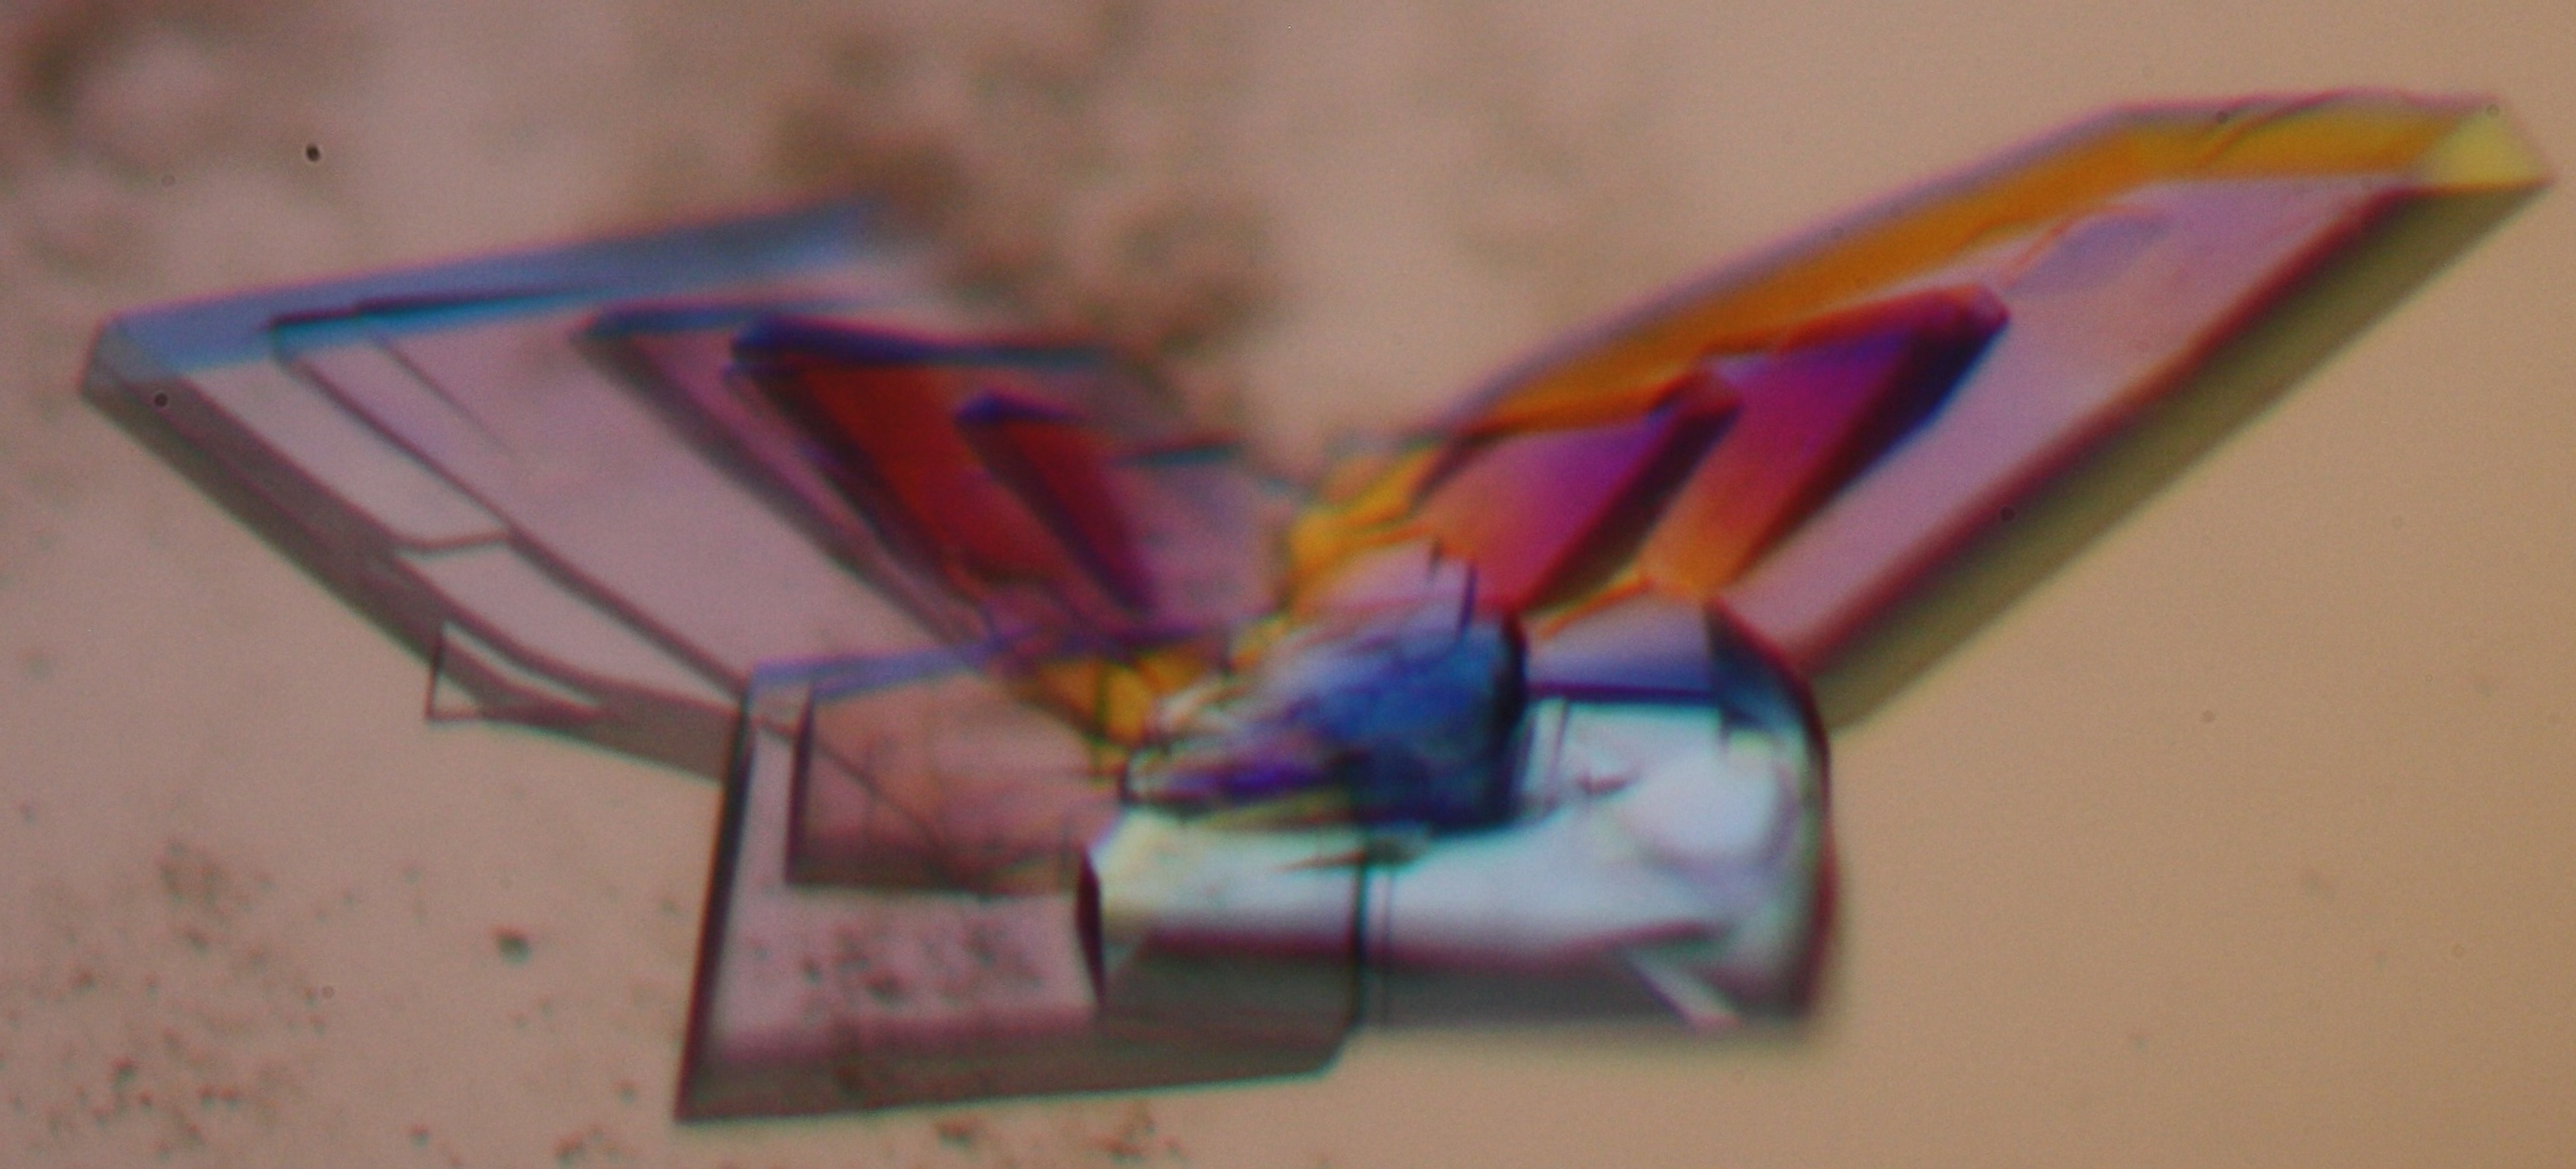
\includegraphics[width=0.7\textwidth]{crystal_chapter/img/bigflowerxtal.jpg}
   	\end{center}
   	\caption[Example of a large cluster of `plate' RsaA \del 0--222 crystals]{An example of a large cluster of `plate' crystals of RsaA \del 0--222. The cluster was just over one millimeter in width from tip to tip. The largest crystal, on the right, was broken off and diffracted using synchrotron radiation, resulting in disappointing resolution. The color is imparted by a polarizing filter on the microscope, the crystals are naturally colourless.}
   	\label{fig:crystal-flower}
\end{figure}

\subsection{Crystallization of RsaA \del{}0--222 GSCC723} \label{sec:cryst-rsaa-del0}

RsaA \del 0--222 GSCC723 readily crystallized in the successful conditions used for RsaA \del 0--222. However, the crystals that formed had a different morphology. The crystals looked dendritic, like trees or snowflakes. Extensive optimizations were performed to improve the shape and size of the crystals but no improved conditions could be found. The final conditions used were 9\% \ac{peg}, 100 \millimolar{} tris pH 7.4, and 150 \millimolar{} \ce{SrCl2}. The protein concentration was 3.5 \mgperml{}, 6 \microlitre{} of protein solution was mixed with 3 \microlitre{} of mother liquor. 

A few of the dendritic crystal clusters had branches that were clean, individual crystals. In those cases, the crystal branches were gently broken off of the main cluster and used for X-ray diffraction.


\subsection{Data collection and processing}\label{sec:crystal-data-collection}
X-ray diffraction data was collected, multiple times, at two synchrotron light
sources: the \ac{cls} in Saskatoon, Saskatchewan and \ac{ssrl} at Stanford
University, California. Both facilities proved suitable for our data collection
needs. The beamlines at \ac{cls} offered a slightly larger spectrum of available
X-ray wavelengths; some of the high energy wavelengths proved useful for
accessing the K-edges of strontium (0.7699 \AA) and bromine (0.9202 \AA). For
our best diffracting crystal, diffraction was performed at the `CMCF 08ID-1'
beamline at \ac{cls}. A wavelength of 1.54 \AA (equal to the copper K-edge) was
used to maximize the overall anomalous signal of iodide.  As
reference, \cref{fig:edges} shows theoretical anomalous scattering coefficients
for most of the elements used in this study. Data were processed using
HKL3000\upcite[]{minor2006hkl} or XDS\upcite[]{kabsch2010xds} ( see
\cref{tab:diffractiondata}); phasing attempts were performed using
Shelx\upcite[]{sheldrick2010experimental} or AutoSol in
Phenix\upcite[.]{adams2010phenix} Data were collected through a full
360$\circ$ of rotation, due the low symmetry found in the `plate' crystals

\begin{figure}[htb]
  	\begin{center}
   		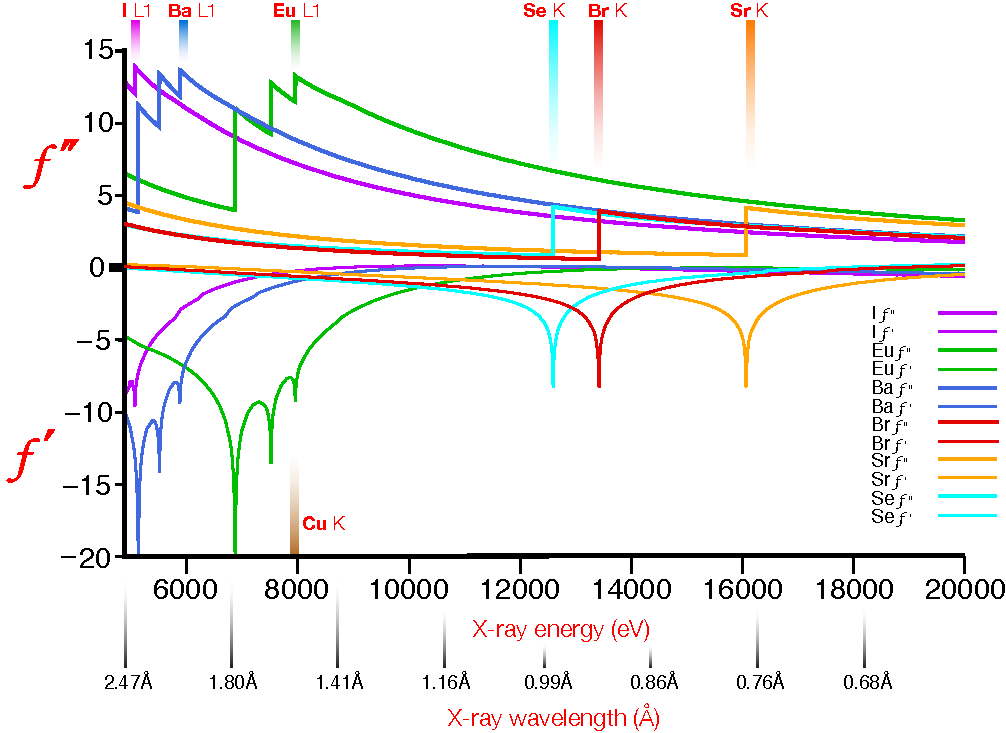
\includegraphics[width=\textwidth]{crystal_chapter/img/edgeplots.pdf}
   	\end{center}
   	\caption[Edge plots for useful anomalous dispersion elements]{
   	Theoretical plots of anomalous scattering coefficients for various elements used in this study. The K-edges and L1-edges that are present within the range of this graph were indicated. Selenium was included because it is often used as a landmark to compare with other elements.}
   	\label{fig:edges}
\end{figure}    

\section{Results}\label{sec:crystal-results}

\subsection{Initial crystallization and optimization}\label{sec:init-cryst-optim} 
 Attempts to crystallize RsaA \del 0--222 started with the pre-assembled crystallization screens \ac{jcsg} Core I, II, III, and IV. Higher protein concentrations were sought because it is generally believed that higher protein concentrations would lead to better results and literature sources recommended protein concentration ranges centering on 10 \mgperml\upcite[.]{jancarik1991sparse}  The RsaA \del 0--222 truncate was readily concentrated to 5--7 \mgperml, but when concentrated beyond 7--9 \mgperml aggregation began to occur, either visual macroaggregation or microaggregation assessed by \ac{dls}. Initial screens were assembled at 9 \mgperml, small crystalline shapes were observed after one week at room temperature. Those first crystals grew in JCGS Core I, well 28 with conditions of 20\% \ac{peg} 8000, 200 \millimolar \ce{MgCl2}, and 100 \millimolar Tris pH 7.
 
The first attempts to transfer from a sitting-drop strategy, as used in initial screening, to a hanging-drop strategy, to be used in optimization, were unsuccessful due to widespread protein precipitation/aggregation. Shifting our divalent cation from \ce{Mg^2+} to \ce{Ca^2+} led to small crystals in our drops. Crystals that were grown with \ce{Ca^2+} were very thin, but sizable ($>$0.5 \si{\milli\meter}) in the other two dimensions. The biggest improvements came from shifting the cation again to \ce{Sr^2+} and lowering the concentrations of the protein and precipitants. Due to low protein concentrations, larger drop sizes (6--10 \microlitre) were utilized and larger ratios between protein and mother liquor were (1.5:1--3:1) used so that initial conditions would not cause protein precipitation but protein concentrations would eventually get high enough to be supersaturated. Fine tuning of protein concentration and drop ratios were mostly used to optimize nucleations in the drops. RsaA \del 0--222 always nucleated well, leading to more drops full of small crystals than clear drops with no crystals. A protein concentration in the range of 3.5--4.5 \mgperml, mixed in a ratio of 1.5:1 with mother liquor, had the best results, averaging around 3 nucleations per drop. Further optimization to the crystallization conditions, such as lowering salt concentration (200 \millimolar to 150 \millimolar) and raising the pH (7 to 7.4), were of arguable efficacy. 

\subsection{Properties of the RsaA \del 0--222 crystals}\label{sec:properties-crystals}
Our first diffracting crystals of RsaA \del 0--222 were `plate' crystals having a rhomboid shape.  \Cref{fig:crystal-panel} shows examples of these rhomboid crystals. The proportional dimensions of the crystals roughly match the relative dimensions of the crystal unit cell (see \Cref{tab:diffractiondata}), although the thickness seemed variable. The crystals grew often as clusters or stacks, which did not aid in diffraction. \Cref{fig:crystal-flower} on \cpageref{fig:crystal-flower} shows one example of how many of these crystal clusters appeared. The rhomboid `plate' crystals were very strong, resisting crushing so well that we were initially concerned that they were salt crystals. The `plates' also resisted X-ray induced damage well---often diffracting acceptably well after two or three full data collections. 

Later crystallization efforts for RsaA \del 0--222 started to yield crystals that were not rhomboid, rather they were hexagonal prisms, like pencils. Drops identical to and next to drops producing `plate' crystals would often grow `pencil' crystals. A few drops even produced both `plate' crystals and `pencil' crystals. These `pencil' crystals looked like protein crystals under a polarizing filter on the microscope and they were confirmed to be protein by X-ray diffraction. The `pencil' crystals were very fragile and often broke or cracked under gentle manipulation. The `pencils' grew as solitary crystals often on contact with the lower surface of the crystallization drop. \Cref{fig:pencils} shows a few examples of the hexagonal prism crystals of RsaA \del 0--222.

Low pH solutions would readily crack and destroy any form RsaA \del 0--222 crystal. Unfortunately, this pH limitation precluded us from using some soaking agents like uranium compounds and higher concentrations of tantalum bromide. The `plate' crystals were generally more stable in soaking conditions with high salt concentrations than the `pencil' crystals. The `pencil' crystals would quickly crack in high concentrations of \ce{KI} and \ce{KBr}.

\begin{figure}[htb]
  	\begin{center}
   		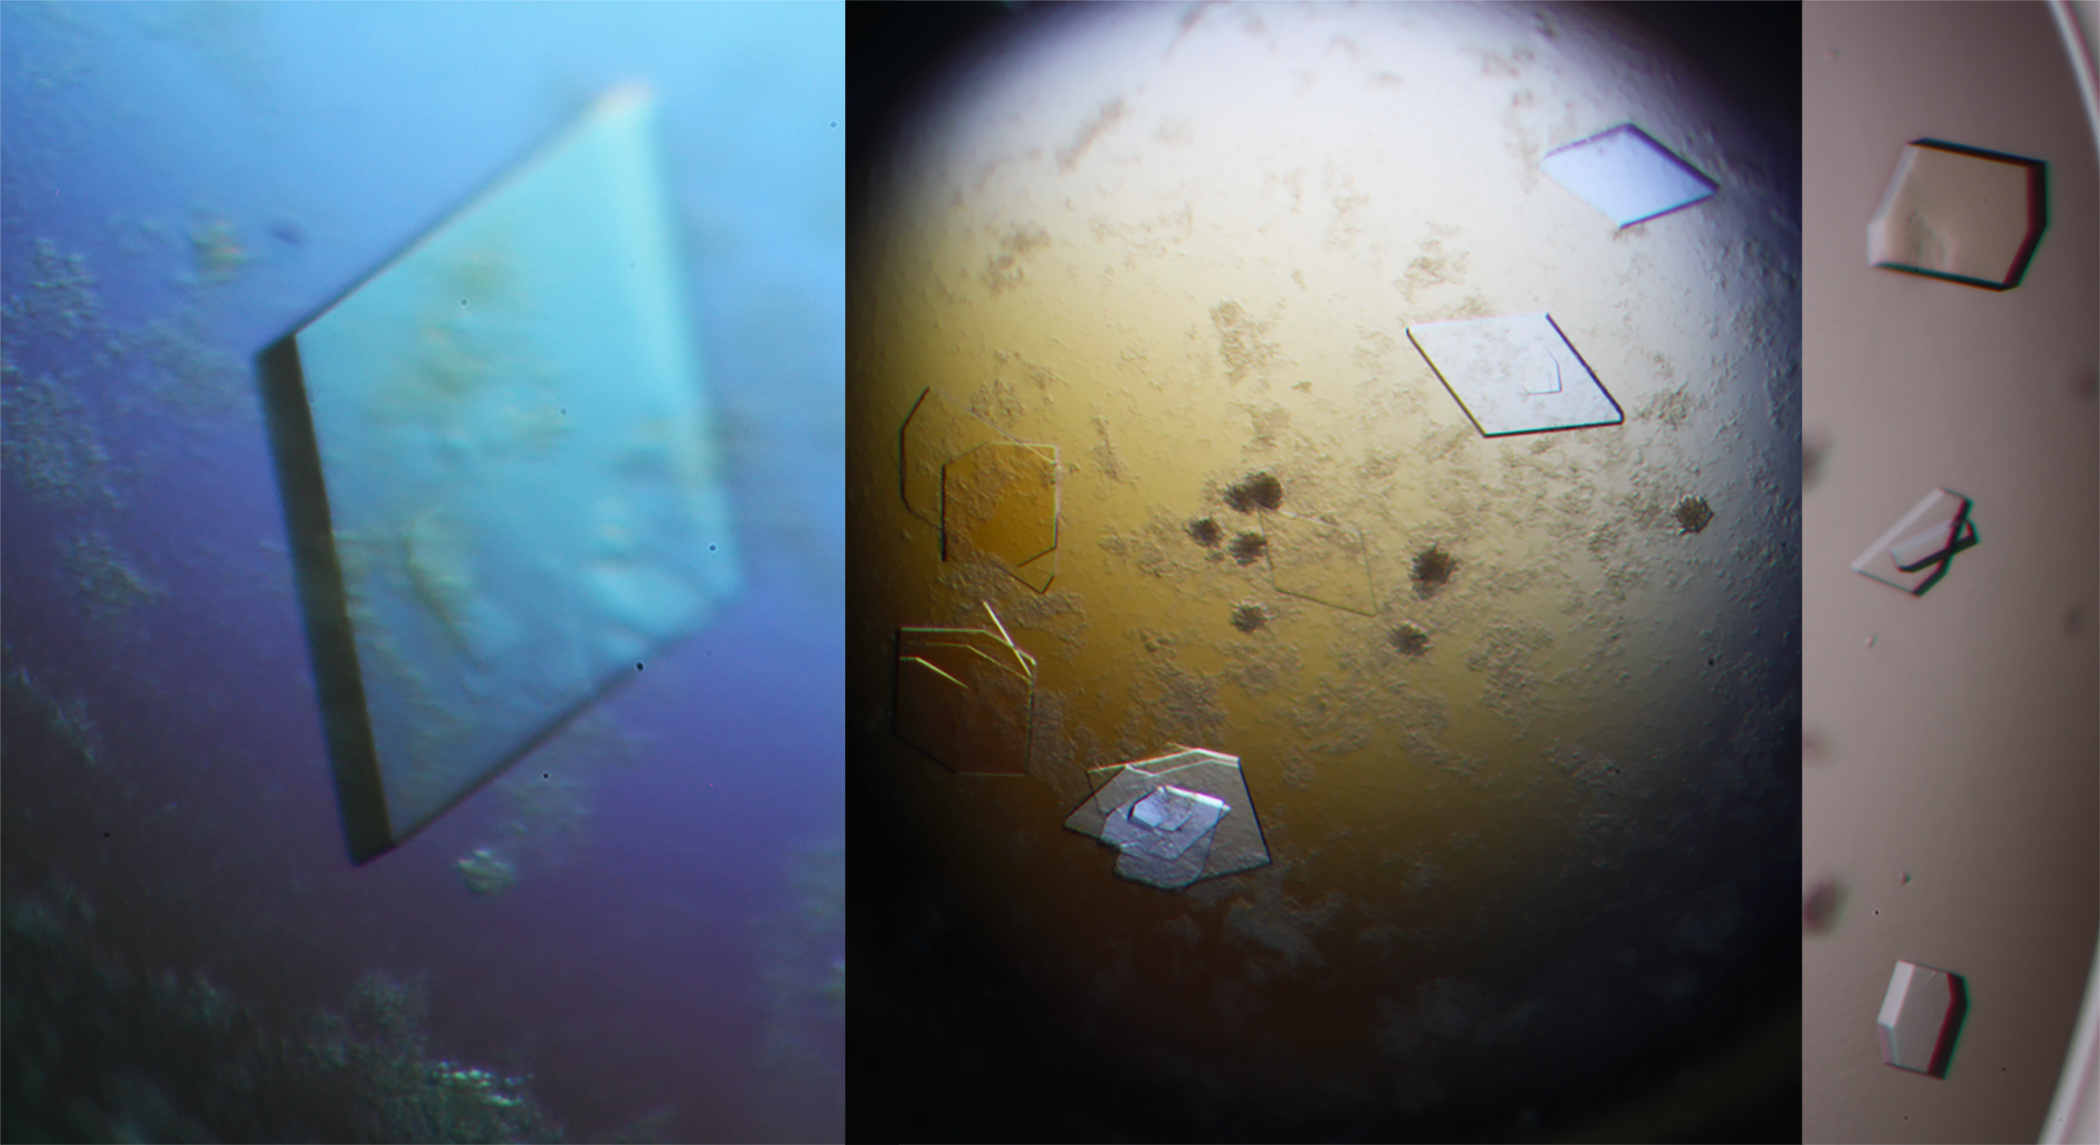
\includegraphics[width=0.9\textwidth]{crystal_chapter/img/goodxtal.jpg}
   	\end{center}
   	\caption[Panel of well diffracting `plate' crystals of RsaA \del 0--222]{A panel of `plate' crystals of RsaA \del 0--222. The left figure show an individual crystal with the common rhomboid shape and relatively thin width. The center figure shows a wide-view of a drop containing multiple `plate' crystals. The right figure shows three crystals of RsaA \del 0--222 that were grown in the presence of 5 \millimolar{} \ce{EuNO3}. The color in the first two images is imparted by a polarizing filter on the microscope, the crystals are naturally colourless. The colour of the right figure is unadjusted and representative of the natural colour of the crystals.}
   	\label{fig:crystal-panel}
\end{figure}   
\begin{figure}[htb]
  	\begin{center}
   		\includegraphics[width=0.9\textwidth]{crystal_chapter/img/pencils.pdf}
   	\end{center}
   	\caption[A panel of `pencil crystals of RsaA \del 0--222']{A panel of `pencil crystals of RsaA \del 0--222. The left figure shows how some of the `pencils' grew in the presence of `plate' crystals, note the `plates' in that panel were not suitable for X-ray diffraction. The right figure highlights a particularly large `pencil' crystal. These crystals were very fragile.  The color in the images is imparted by a polarizing filter on the microscope, the crystals are naturally colourless.} 
   	\label{fig:pencils}
\end{figure}   

\subsection{Properties of the RsaA \del 0--222 GSCC723 crystals}\label{sec:properties-rsaa-del}
As mentioned before, the only crystals that were formed when using the RsaA \del 0--222 GSCC723 protein were `dendritic' crystals that resembled trees or snowflakes. \Cref{fig:crystal-dendrites} shows a few examples of these crystals. Most of these crystals were too clustered to be useful for diffraction but a few of the clusters had branches that could be removed and used for diffraction. \Cref{fig:nice-trees} shows a few of the dendritic clusters that were broken apart and diffracted. 

The RsaA \del 0--222 GSCC723 crystals had similar properties to the RsaA \del 0--222 `plate' crystals; the GSCC723 crystals were very strong and stable in most soaking conditions. Unfortunately due to the poor diffraction, the GSCC crystals' potential ability to bind more phasing ions was never realized.

\begin{figure}[htb]
  	\begin{center}
   		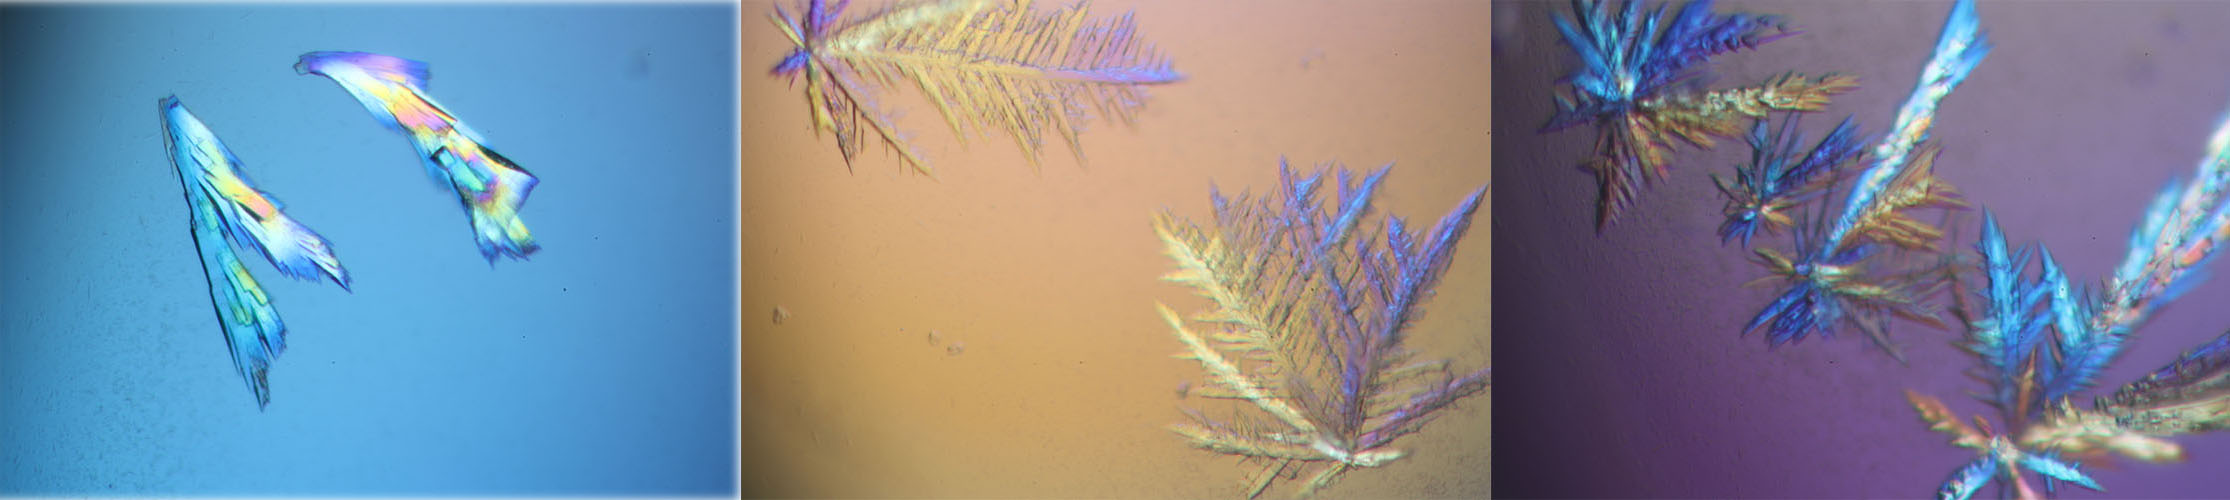
\includegraphics[width=0.9\textwidth]{crystal_chapter/img/dendroXtals.jpg}
   	\end{center}
   	\caption[Examples of unusable `dendritic' RsaA \del 0--222 GSCC723 crystals]{Examples of `dendritic' crystals formed when the RsaA \del 0--222 GSCC723 protein construct was crystallized. The color is imparted by a polarizing filter on the microscope, the crystals are naturally colourless.}
   	\label{fig:crystal-dendrites}
\end{figure}

\begin{figure}[htb]
  	\begin{center}
   		\includegraphics[width=0.9\textwidth]{crystal_chapter/img/nicetrees.pdf}
   	\end{center}
   	\caption[`Dendritic' RsaA \del 0--222 GSCC723 crystals that were used for X-ray diffraction]{A panel of better `dendritic' crystals of RsaA \del 0--222 GSCC723. These are examples of some of the GSCC723 crystals having branches that were suitable for X-ray diffraction. A few of the side crystals were broken off and used for diffraction.  The color in the images is imparted by a polarizing filter on the microscope, the crystals are naturally colourless. The colour of the right figure is unadjusted and representative of the natural colour of the crystals.}
   	\label{fig:nice-trees}
\end{figure}   

\subsection{X-ray diffraction and phasing}\label{sec:x-ray-diffraction}

The biggest issue that we have had to deal with in this crystallography has been the variability of the crystals. The majority of the crystals of RsaA that have been grown have very poor X-ray diffraction. Frustratingly, there was not an effective way to predict which crystal would diffract well. Our best results came from a large crystal that was relatively thin---two features that seemed to be important because small crystals did not diffract well and overly thick crystals were plagued with smeared, messy reflections. \Cref{fig:diffraction} shows one frame of data from our best dataset. An interesting aspect of the data, specifically from `plate' and `dendrite' crystals, is the anisotopy we observe in our diffraction. Due to the often poor quality of the data, we would always collect our data through 360$\circ$ which would lead to long collection strategies and increased radiation damage to the crystal. Radiation damage was never too much of an issue though, as the `plate' crystals were remarkably resistant to damage. Table \ref{tab:diffractiondata} gives an overview of the X-ray diffraction data.

        \begin{table}[p]
            \caption[Summary data from our X-ray diffraction of RsaA \del 0--222]{ }
            \begin{center}
                \begin{tabular}{@{}ll@{}}
                    \toprule
										\multicolumn{2}{c}{RsaA \del 0--222}			 \\ \midrule
										Space group				& P2$_{1}$							 \\
										Cell dimensions		&												 \\
										a, b, c (\AA)				& 210.79, 80.74, 221.9	 \\
										$\beta$ ($\circ$)							& 117.46								 \\
										Resolution (\AA)		& 50.00--2.50 (2.54--2.50) \\
										R$_{merge}$				& 0.13 (0.54)						 \\
										I / $\delta$I						 & 13.7 (2.8)							\\
										Completeness (\%) & 99.8 (97.6)						\\
										Redundancy				& 3.8										 \\ \bottomrule
               \end{tabular}
            \end{center}
            \label{tab:diffractiondata}
        \end{table}   
 
 Once we had crystals that diffracted to a suitable extent the final step in generating an electron density map would be phasing. Molecular replacement strategies were not possible due to a lack of homologous structures in the Protein Data Bank. The \ac{rtx}  motifs in RsaA provide a tempting region for structural homology, such as the structure in \cref{fig:intro-rtx} (on \cpageref{fig:intro-rtx}). Neither the structures of solved \ac{rtx} motifs as molecular replacement  nor the generated Phyre\upcite[]{kelley2015phyre2} structure for RsaA's \ac{rtx} motifs were effective molecular replacement search models. To try and solve the phase problem we turned to the X-ray fluorescence techniques of \ac{MAD} and \ac{SAD}. 

Our main two candidates for \ac{MAD}/\ac{SAD} phasing elements were the halides, iodine and  bromine\upcite[.]{dauter2000novel} These halides were introduced into the crystals by soaking the crystals in \ce{KI} and \ce{KBr}. Iodine does not have an accessible K or L edge but provides a \ac{SAD}  suitable anomalous signal at achievable wavelengths. Refer back to \cref{fig:edges} for the theoretical profiles of anomalous signal. Iodide-soaked `plate' crystals, among the first conditions ever tested, diffracted well and anomalous signal could be detected in their datasets but not enough to allow for densities to be calculated. A great deal of effort went into trying to improve our initial datasets with more of an anomalous component from iodide. Very few subsequent iodide-soaked crystals diffracted at all  and those that did were of low resolution. Bromine has an accessible K$_{a}$ edge at 0.9202 \AA and so it is useful for \ac{MAD}. Unlike iodide, bromide-soaked crystals did not have the high rate of crystals  with no diffraction but like iodide, few bromide-soaked crystals diffracted beyond 4 \AA{}. 

Many other phasing compounds were tested. The lanthanides all provide a strong  anomalous signal and have been successfully used in the past for \ac{SAD}\upcite[.]{baranova2012sbsb} Lanthanum, Lutetium, and Europium were all used as soaking agents but none produced any detectable anomalous dispersion in the resulting datasets. Europium was also successfully used in the mother-liquor of the crystals to be co-crystallized. Unfortunately, the co-crystallized crystals had no detectable anomalous signal, despite good diffraction. Europium's L$_{1}$ edge is accessible with synchrotron radiation (see \cref{fig:edges}), \ac{MAD} fluorescence scans were done to confirm that there was no detectable Europium in the crystals. \Cref{fig:crystal-panel} features a few of the Europium co-crystallized crystals. In the vein of co-crystallization, Strontium and Barium were effective components of the mother liquor, and possibly potent phasing elements, but neither provided an effective solution to the phase problem when tried. The more exotic compounds Tantulum bromide (\ce{Ta6Br12}) and  triiodide were also tried without resulting in the necessary data. 
 
\begin{figure}[htb]
  	\begin{center}
   		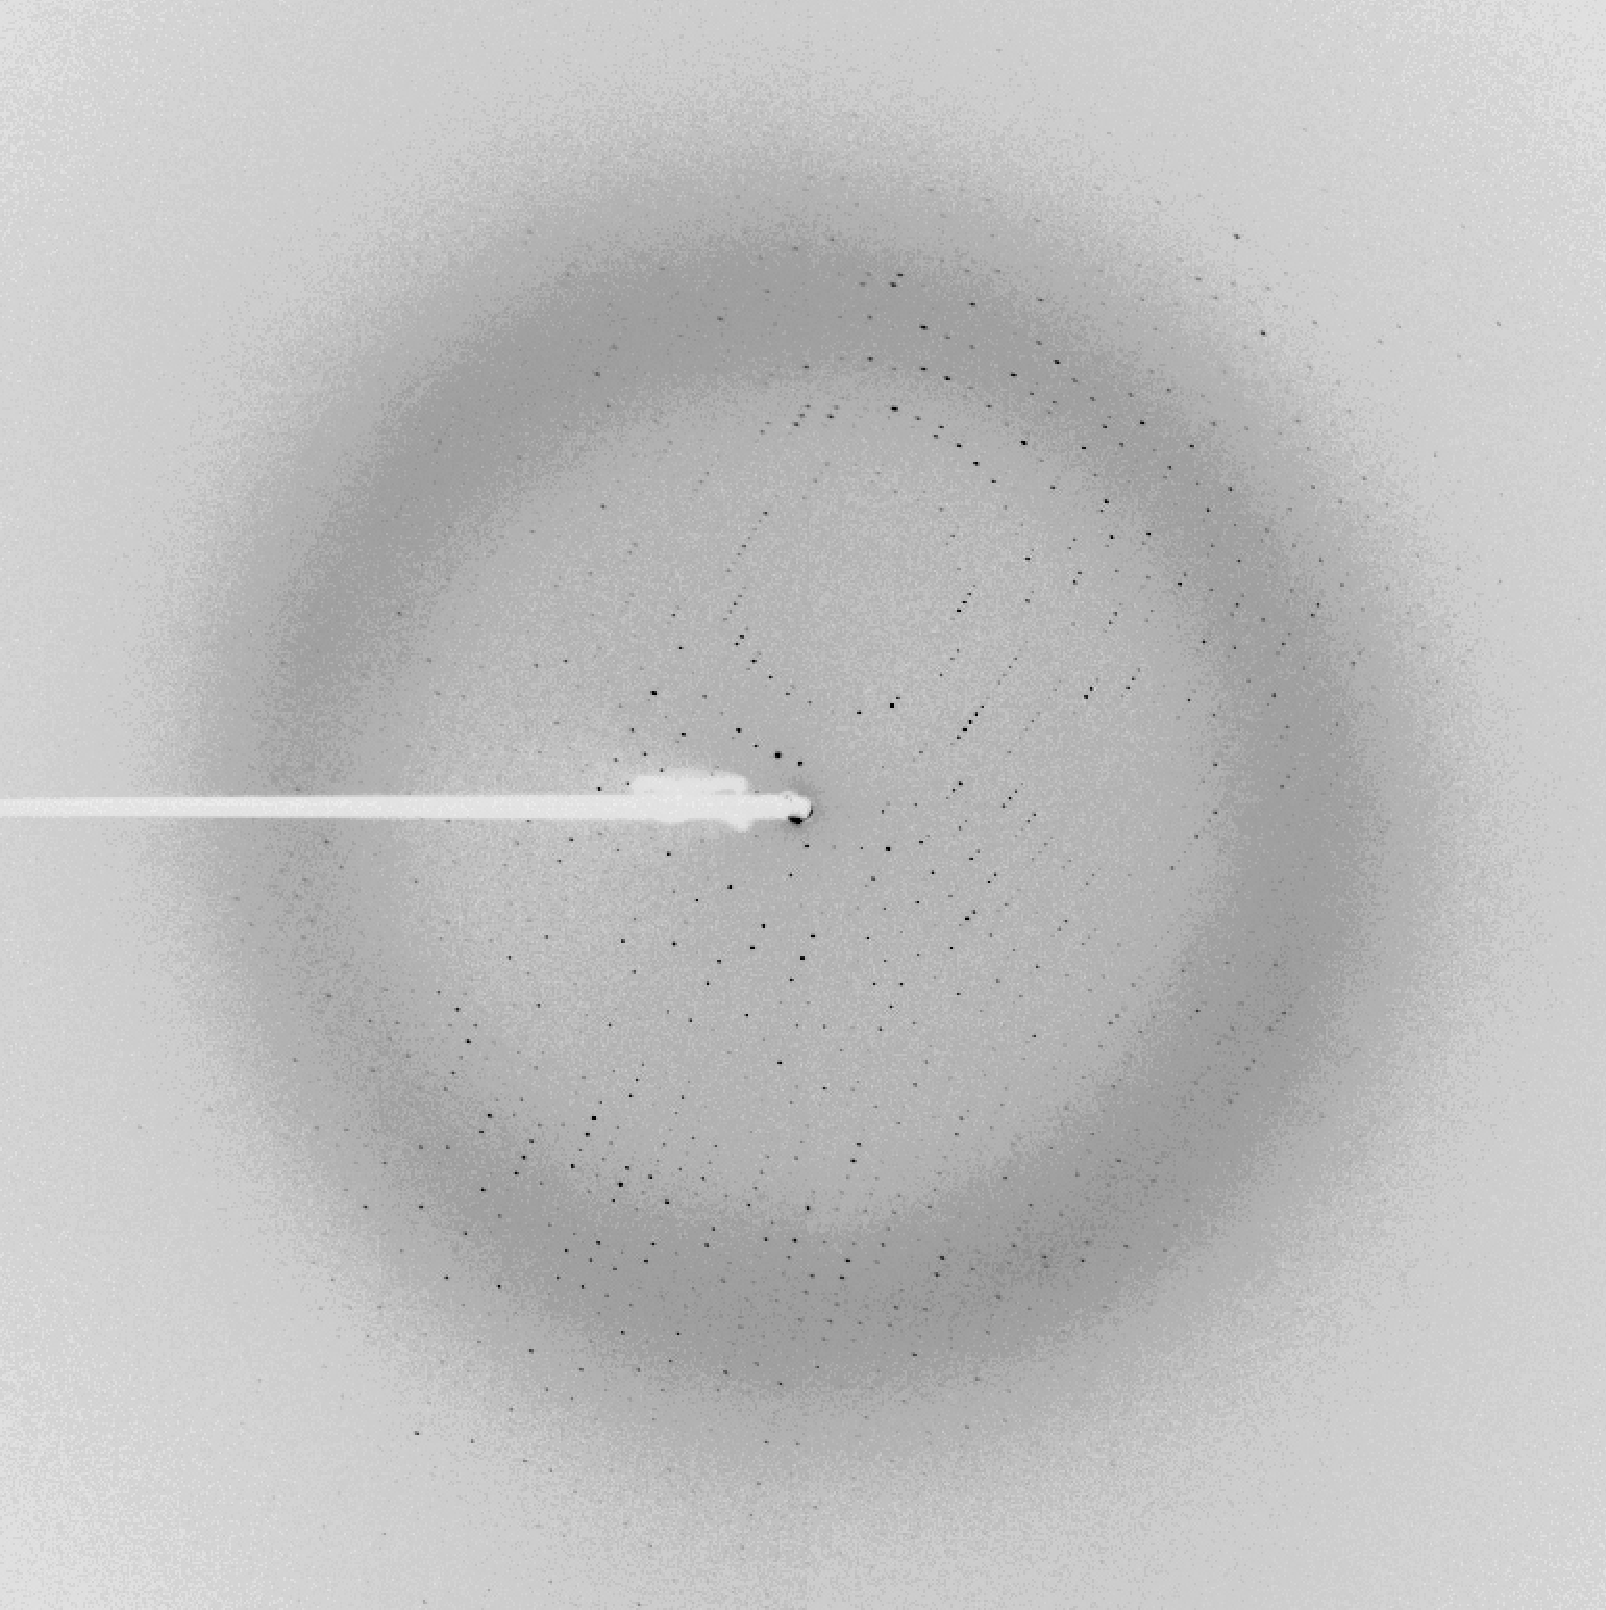
\includegraphics[width=0.9\textwidth]{crystal_chapter/img/rsaadiffraction.pdf}
   	\end{center}
   	\caption[A diffraction pattern of RsaA \del 0--222, `plate' crystal]{This figure shows a frame from a X-ray diffraction data collection. 
This crystal was a large `plate' crystal that was our best diffracting crystal to date. The crystal was soaked in 0.5
 \si{\molar} 
\ce{KI} 
for 30 sec. The wavelength of the incident X-ray beam was set to 1.541 \AA{} (the copper K$_{a}$ edge). Theoretical resolution from this data would have been 2.50 \AA{} if there had been enough anomalous signal to use in \ac{SAD} phasing. Notice the anisotropy in diffraction, \ie the spots reach further from the center to the upper right and lower left.}
   	\label{fig:diffraction}
\end{figure}   

There were only ever a few `dendritic' crystals that were suitable for X-ray diffraction and none of those few diffracted to an extent or in a manner that was conducive to solving the structure of RsaA \del 0--222 GSCC723. One `dendritic' crystal did diffract reliably to 3.5 \AA{} but exhibited multiple overlapping signals, probably due to separate crystals being fused together.  

The `pencil' crystals never diffracted to any significant extent, at most to 6--10 \AA{}. Initial processing of one of the `pencil' diffraction patterns suggested that its space group was P6. A P6 space group has higher symmetry than the P2$_{1}$ space group we observed in our `plate' crystals. We had hopes that the higher symmetry would provide better quality data, unfortunately no well performing `pencil' crystals were ever isolated. The only pencil that we did try to perform a complete data collection on quickly lost diffraction due to radiation damage.

\section{Discussion}\label{sec:crystal-discussion}
Our protein construct, RsaA \del 0--222, was expressed our in \caulobacter protein expression system\upcite[.]{bingle1997expression, UmeloNjaka20011406, Bingle1990143} All attempts to produce protein in \ecoli{} resulted in highly insoluble inclusion bodies that resisted refolding (data not shown). Expression levels of RsaA in its native host is notably high\upcite[]{lau2010analysis} but the system did not initially produce protein in an appropriate form. The problem of aggregation persisted in \caulobacter secreted RsaA; the problem was assuaged by the N-terminal deletion construct, RsaA \del 0--222, but was only completely solved when we started to culture the cells without agitation in wide, shallow flasks. Our shallow culture expression system proved successful at producing 130--150 \milligram  of purified, concentrated protein per litre of culture supernate. RsaA is the natural product of \caulobacter but this system could be useful in producing exogenous protein for crystallization by fusion to the required type 1 section signal\upcite[.]{bingle2000secretion}

The reasons for an N-terminal truncation of RsaA are two-fold; deletion of the
N-terminus produces protein that no longer anchors itself to outer membrane,
resulting in free-secreted supernatant protein and the N-terminus has been
identified as the center of three-fold symmetry (Amat et al., 2010). Therefore,
its deletion results in soluble protein that no longer leads to wide-scale
\ac{S-layer} formation or aggregation and is freely secreted into the
supernatant. The success of structurally characterizing any S-layer protein impinges upon overcoming such issues and our strategies resulted in large well-diffracting crystals.

Our `plate' crystals diffracted to 2.5 \AA{} with unit-cell parameters of
a=210.79 \AA, b=80.74 \AA, c=221.9 \AA,  and $\beta$=117.46 degrees. These
crystal unit-cell sizes almost exactly match the 2D unit size of native
\ac{S-layer} repeating unit, a hexamer of RsaA monomers\upcite[.]{smit1992s}
These results suggest that the unit-cell of our crystals is six copies of RsaA
\del 0--222, corresponding to a solvent content of  about 60\%. Our hexagonal
columnar crystals have never diffracted to a suitable resolution, but they are
promising because they have higher symmetry and that may result in improved
datasets. As our protein has no close matches in the structural databases to use
for the purposes of molecular replacement, solving the phase problem was
attempted with iodine derivitization with \ac{SAD} and bromide with \ac{MAD}.
Neither of these approaches gave us the required anomalous data that we would
need for a solution.   RsaA does not have many charged amino acids, even after
we installed the GSCC cassette, and that is why the halides have been so
strongly pursued; they do not require specific residues for
activity\upcite[.]{dauter2000novel} Patterson analysis of the dataset suggests issues with
pseudotranslational symmetry confounding phasing attempts, with the largest
Patterson peak at a height of about 30\%.  Twinning analyses indicate that no twinning is suspected.

As of this writing, the crystallography portion of this work is still ongoing. We are so close to completing this effort that it is hard to imagine that a solution does not exist.  The fact remains that we have developed techniques to crystallize the \ac{S-layer} protein and generally that is the most important step in a crystallization project. To conclude this chapter, below is a quote from Alexander McPherson's 2004 review on macromolecular crystallography:\upcite[]{mcpherson2004introduction}

\begin{quote}
 Presently, and in the foreseeable future, the only technique that can yield atomic level structural images of biological macromolecules is X-ray diffraction analysis as applied to single crystals. While other methods may produce important structural and dynamic data, for the purposes described above, only X-ray crystallography is adequate. As its name suggests, application of X-ray crystallography is absolutely dependent on crystals of the macromolecule, and not simply crystals, but crystals of sufficient size and quality to permit accurate data collection. The quality of the final structural image is directly determined by the perfection, size, and physical properties of the crystalline specimen, hence the crystal becomes the keystone element of the entire process, and the ultimate determinant of its success.
\end{quote}